\part{À chacun sa culture qui fait rêver}
\chapter{Le Brésil}

\begin{center}
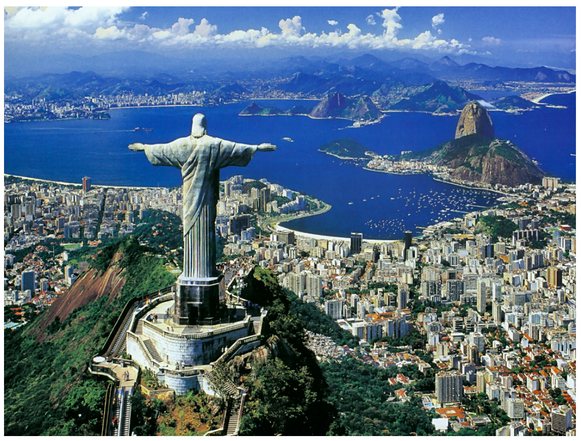
\includegraphics[scale=0.5]{bresil1.png}
\end{center}

\section{Une présentation sommaire}

\paragraph{} En juillet dernier, je mettais les pieds en Amérique du Sud pour
la seconde fois de mon existence. Après la Colombie, le Brésil. La période
choisie était plutôt atypique puisque j'étais arrivé à Rio de Janeiro deux
jours avant la fameuse victoire de l'Allemagne sur le pays hôte. Un match que
j'avais d'ailleurs pu suivre sur le sable de Copacabana. Jusqu'à la mi-temps.
Une grande partie de la foule brésilienne refusa la douche tiède après la
froide et rentra chez elle.

\paragraph{} Dans la culture moderne, on associe très rapidement taxi avec New
York. Merci Hollywood. Néanmoins, je doute que leurs chauffeurs soient aussi
passionnants que ceux que l'on peut trouver au Brésil.  Le chauffeur de taxi
brésilien peut être très causant, très aimable et faire figure d'excellent
ambassadeur pour son pays.

\section{Un pays de contrastes}

\paragraph{} Le Brésil est un pays de contrastes. Ce sont ses influences
européennes, africaines, et bien évidemment amérindiennes qui, depuis 1822, ont
contribué à modeler le Brésil actuel. Quel autre pays au monde peut se targuer
de posséder une diversité culturelle si riche?

\paragraph{} Plus surprenant par contre, l'attention presque obsessionnelle que
portent certains Brésiliens à leur corps, opposé à d'autres qui s'ouvrent une
voie royale vers un diabète de type 2. Le contraste est particulièrement
saisissant lorsque vous vous promenez sur le trottoir qui sépare la plage de
Copacabana de l'Avenida Atlântica. En effet, athlètes avertis et obèse se
mélangent volontiers sur ces quelque 4,5 km de pavés noirs et blancs. Mais pour
différentes raisons. Les premiers, à pied ou à vélo, viennent ici pour se
dépenser et sculpter leur corps, mais cela est normal dans une ville où le
bikini est à la mode de janvier à décembre. En plus, la ville de Rio de Janeiro
développe depuis 2010 un concept plutôt original matérialisé par la présence
d'une quarantaine d'instruments de musculation le long de ses plages. Les
autres, les bons vivants, se baladent à un rythme plus décontracté et
n'hésitent pas à se laisser tenter par les gourmandises proposées par les
dizaines de bars circulaires qui jonchent les abords de la plage.

\begin{center}
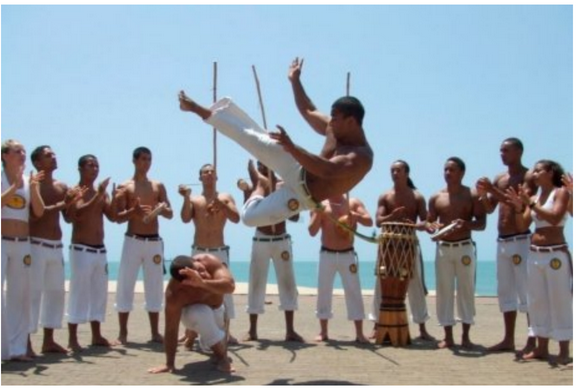
\includegraphics[scale=0.5]{bresil2.png}
\end{center}

\section{Une tradition culturelle}

\paragraph{} La tradition culturelle brésilienne est extrêmement riche et
variée grâce à son fort métissage, notamment du point de vue musical (samba,
bossa nova, forró, frevo\ldots), chorégraphique (capoeira) et culinaire
(churrasco, feijoada, caipirinha, guarana\ldots), mais aussi sur le plan religieux
(candomblé) et mythologique.

\paragraph{} Le candomblé est une des religions afro-brésiliennes pratiquées au
Brésil, mais également dans les pays voisins tels que l'Uruguay, le Paraguay,
l'Argentine ou encore le Venezuela. Mélange subtil de catholicisme, de rites
indigènes et de croyances africaines, cette religion consiste en un culte des
orixás, les dieux du candomblé d'origine totémique et familiale, associés
chacun d'entre eux à un élément naturel (eau, forêt, feu, éclair, etc.). Se
basant sur la croyance de l'existence d'une âme propre à la nature.

\begin{center}
	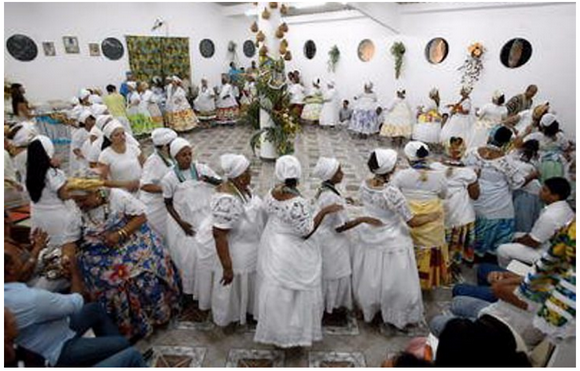
\includegraphics[scale=0.5]{bresil3.png}
\end{center}

\paragraph{} Les danses brésiliennes sont très entraînantes aussi.

\paragraph{} Elle est reconnue dans le monde comme un symbole du Brésil et du
carnaval brésilien. Considérée comme l'une des expressions les plus cultes du
Brésil, la samba fait partie de l'identité nationale brésilienne.

\paragraph{} La samba est un style local au sud et nord du Brésil, en
particulier à Rio de Janeiro, São Paulo, Salvador et Belo Horizonte. Son
importance dans la musique brésilienne traverse toutes les régions du pays,
cependant, des écoles de samba, musiciens de samba et organisateurs de carnaval
centrés sur la performance de la samba se situent partout dans le pays.

\chapter[Les Animes et les Mangas]{Le Japon à travers les Animes et les Mangas}

\section{Introduction}

\paragraph{} Les animes et les mangas ont une place beaucoup plus importante au
Japon qu'en France: par exemple, les animes se regardent en famille font aussi
partie intégrante de la jeunesse japonaise.

\section{Grand public}

\begin{center}
	\centering
	
\includegraphics[scale=0.6]{OnePiece.jpg}
\end{center}

\paragraph{} Parmi les animes et les mangas qui viennent du Japon, ceux qui ont
le plus de chance d'être exportés et vendus dans des pays étrangers, notamment
occidentaux, sont ceux qui touchent le plus grand public. Ils s'agit donc
d'animes ou de mangas dont les thèmes sont internationaux. On compte parmi ces
créations des titres tels que \textit{One Piece}, \textit{Naruto},
\textit{Bleach} qui ont pour thème principal celui de la personne qui est
partie de rien mais qui, au fur et à mesure des efforts réussissent peu à peu à
s'approcher de leur objectif, de la même manière que le ``self-made man''
américain, ce qui est sans doute la raison pour laquelle ces œuvres ont un tel
succès à l'étranger. On trouve aussi des créations comme \textit{Death Note}
qui touche un public un peu plus réduit mais qui prospère de par la fait qu'il
soit dans la catégorie ``suspense''. Il y a aussi bien sûr les films du
studio Ghibli, notamment ceux de \textit{Hayao Miyazaki}, qui ont un succès
remarquable et abordent des thèmes différents et variés.

\section{Petit public}

\begin{center}
	
\includegraphics[scale=0.4]{Clannad.jpg}
\end{center}

\paragraph{} À défaut d'être connus dans le monde entier, les animes  et les
mangas à public réduit sont plus représentatifs et plus explicite par rapport à
la culture japonaise. On y trouve des sujets plus controversés ou qui tiennent
plus à cœur à la population ou à une partie de la population japonaise. Par
exemple, dans l'anime ``\textit{Hataraku Maou Sama}'' ou en anglais ``The devil
is a part-timer'' où il est raconté l'histoire de Satan, employé à temps
partiel dans un équivalent du Mac-Donald, on y observe particulièrement la
vision et la culture japonaise quant au travail et à l'argent. Loin d'être le
seul exemple, on trouve aussi ``Clannad'' qui, dans la deuxième saison,
présente en partie le fait de sortir de l'école et rentrer dans la vie active,
ainsi que le fait d'être parent et ses implications.

\section[Toplist]{Mangas et Animes les mieux notés}

\subsection{Mangas}

\begin{enumerate}
	\item \emph{Berserk}
	\item \emph{Utsuro no Hako to Zero no Maria} (La Boîte du Néant et la 0\ieme Maria)
	\item \emph{Fullmetal Alchemist}
	\item \emph{Watashitachi no Shiawase na Jikan} (Nos Jours Heureux)
	\item \emph{20th Century Boys}
\end{enumerate}

\subsection{Animes}

\subsubsection{Séries}

\begin{enumerate}
	\item \emph{Fullmetal Alchemist: Brotherhood}
	\item \emph{Steins;Gate}
	\item \emph{Gintama'}
	\item \emph{Hunter x Hunter 2011}
	\item \emph{Gintama\degres}
\end{enumerate}

\subsubsection{Longs métrages, courts métrages}

\begin{enumerate}
	\item \emph{Gintama: Kanketsu-hen --- Yorozuya yo Eien Nare} (Gintama: Dernier chapitre --- Demeure Yorozuya)
	\item \emph{Sen to Chihiro no Kamikakushi} (Le Voyage de Chihiro)
	\item \emph{Suzumiya Haruhi no Shoushitsu} (La Disparition de Haruhi Suzumiya)
	\item \emph{Ookami Kodomo no Ame to Yuki} (Les Enfants Loups Ame et Yuki)
	\item \emph{Mononoke Hime} (Princesse Mononoke)
\end{enumerate}
~\\~\\
\noindent
Source: \url{http://myanimelist.net}

\chapter[Matsuris et Croyances]{Le Japon: Matsuris et Croyances}

\section{Les croyances\ldots}

\paragraph{} Le Japon ne possède pas de religion particulière. En effet, les
Japonais auront tendance à se considérer comme appartenant à aucune religion ou
à plusieurs religions en même temps. Les religions principales sont le
shintoïsme et le bouddhisme mais il y a une minorité de chrétiens et de
musulmans.

\paragraph{} Ce mélange de religion est possible grâce aux caractéristiques des
religions principales du pays. Le shintoïsme est une religion polythéiste
tandis que le bouddhisme correspond plus à une philosophie de vie accompagnée
de méditation.

\paragraph{} ``On dit souvent que le Japonais naît, grandit et s'amuse shinto,
s'éduque confucéen, se marie chrétien, vit dans l'irréligion et meurt
bouddhiste''. (Le Japon des Japonais par Philippe PONS et Pierre-François
SOUYRI).

\section[\ldots et les Matsuris]{\ldots à l'origine des Matsuris}

\paragraph{} Le shintoïsme et le bouddhisme sont à l'origine de nombreuses
fêtes traditionnelles autrement appelées Matsuri. En effet, pour attirer la
bienveillance des dieux, chacun d'entre eux est prié et vénéré lors de rituel
et de fête. Bien que les Japonais ne croient pas vraiment en ces dieux, ils
accomplissent ces rituels au cas où les dieux existeraient et retireraient leur
bienveillance envers les Japonais.

\paragraph{} Ces fêtes ont lieu régulièrement tout au long de l'année. Au
printemps, les Japonais fêtent le repiquage du riz et prient pour se protéger
des épidémies. En été, ils prient pour se protéger contre les typhons et les
ravages causés par les insectes ainsi que pour leurs ancêtres.  En hiver, ils
prient pour la nouvelle année. Il y a aussi des fêtes locales pour prier les
dieux locaux à différents moments de l'année.

\paragraph{} Lors de ces festivités, les hommes défilent dans le quartier en
portant le Mikoshi (sorte d'autel portatif) sur leurs dos. Ils sont vêtus d'un
Happi (veste découvrant leur torse) et d'un Fundoshi (sorte de cache-sexe
traditionnel). Une fois l'autel retourné au temple, la fête continu le long de
la rue du temple où l'on peut trouver des stands de friandises en sucres, de
nouilles sautées, de porte-bonheurs\ldots

\begin{center}
	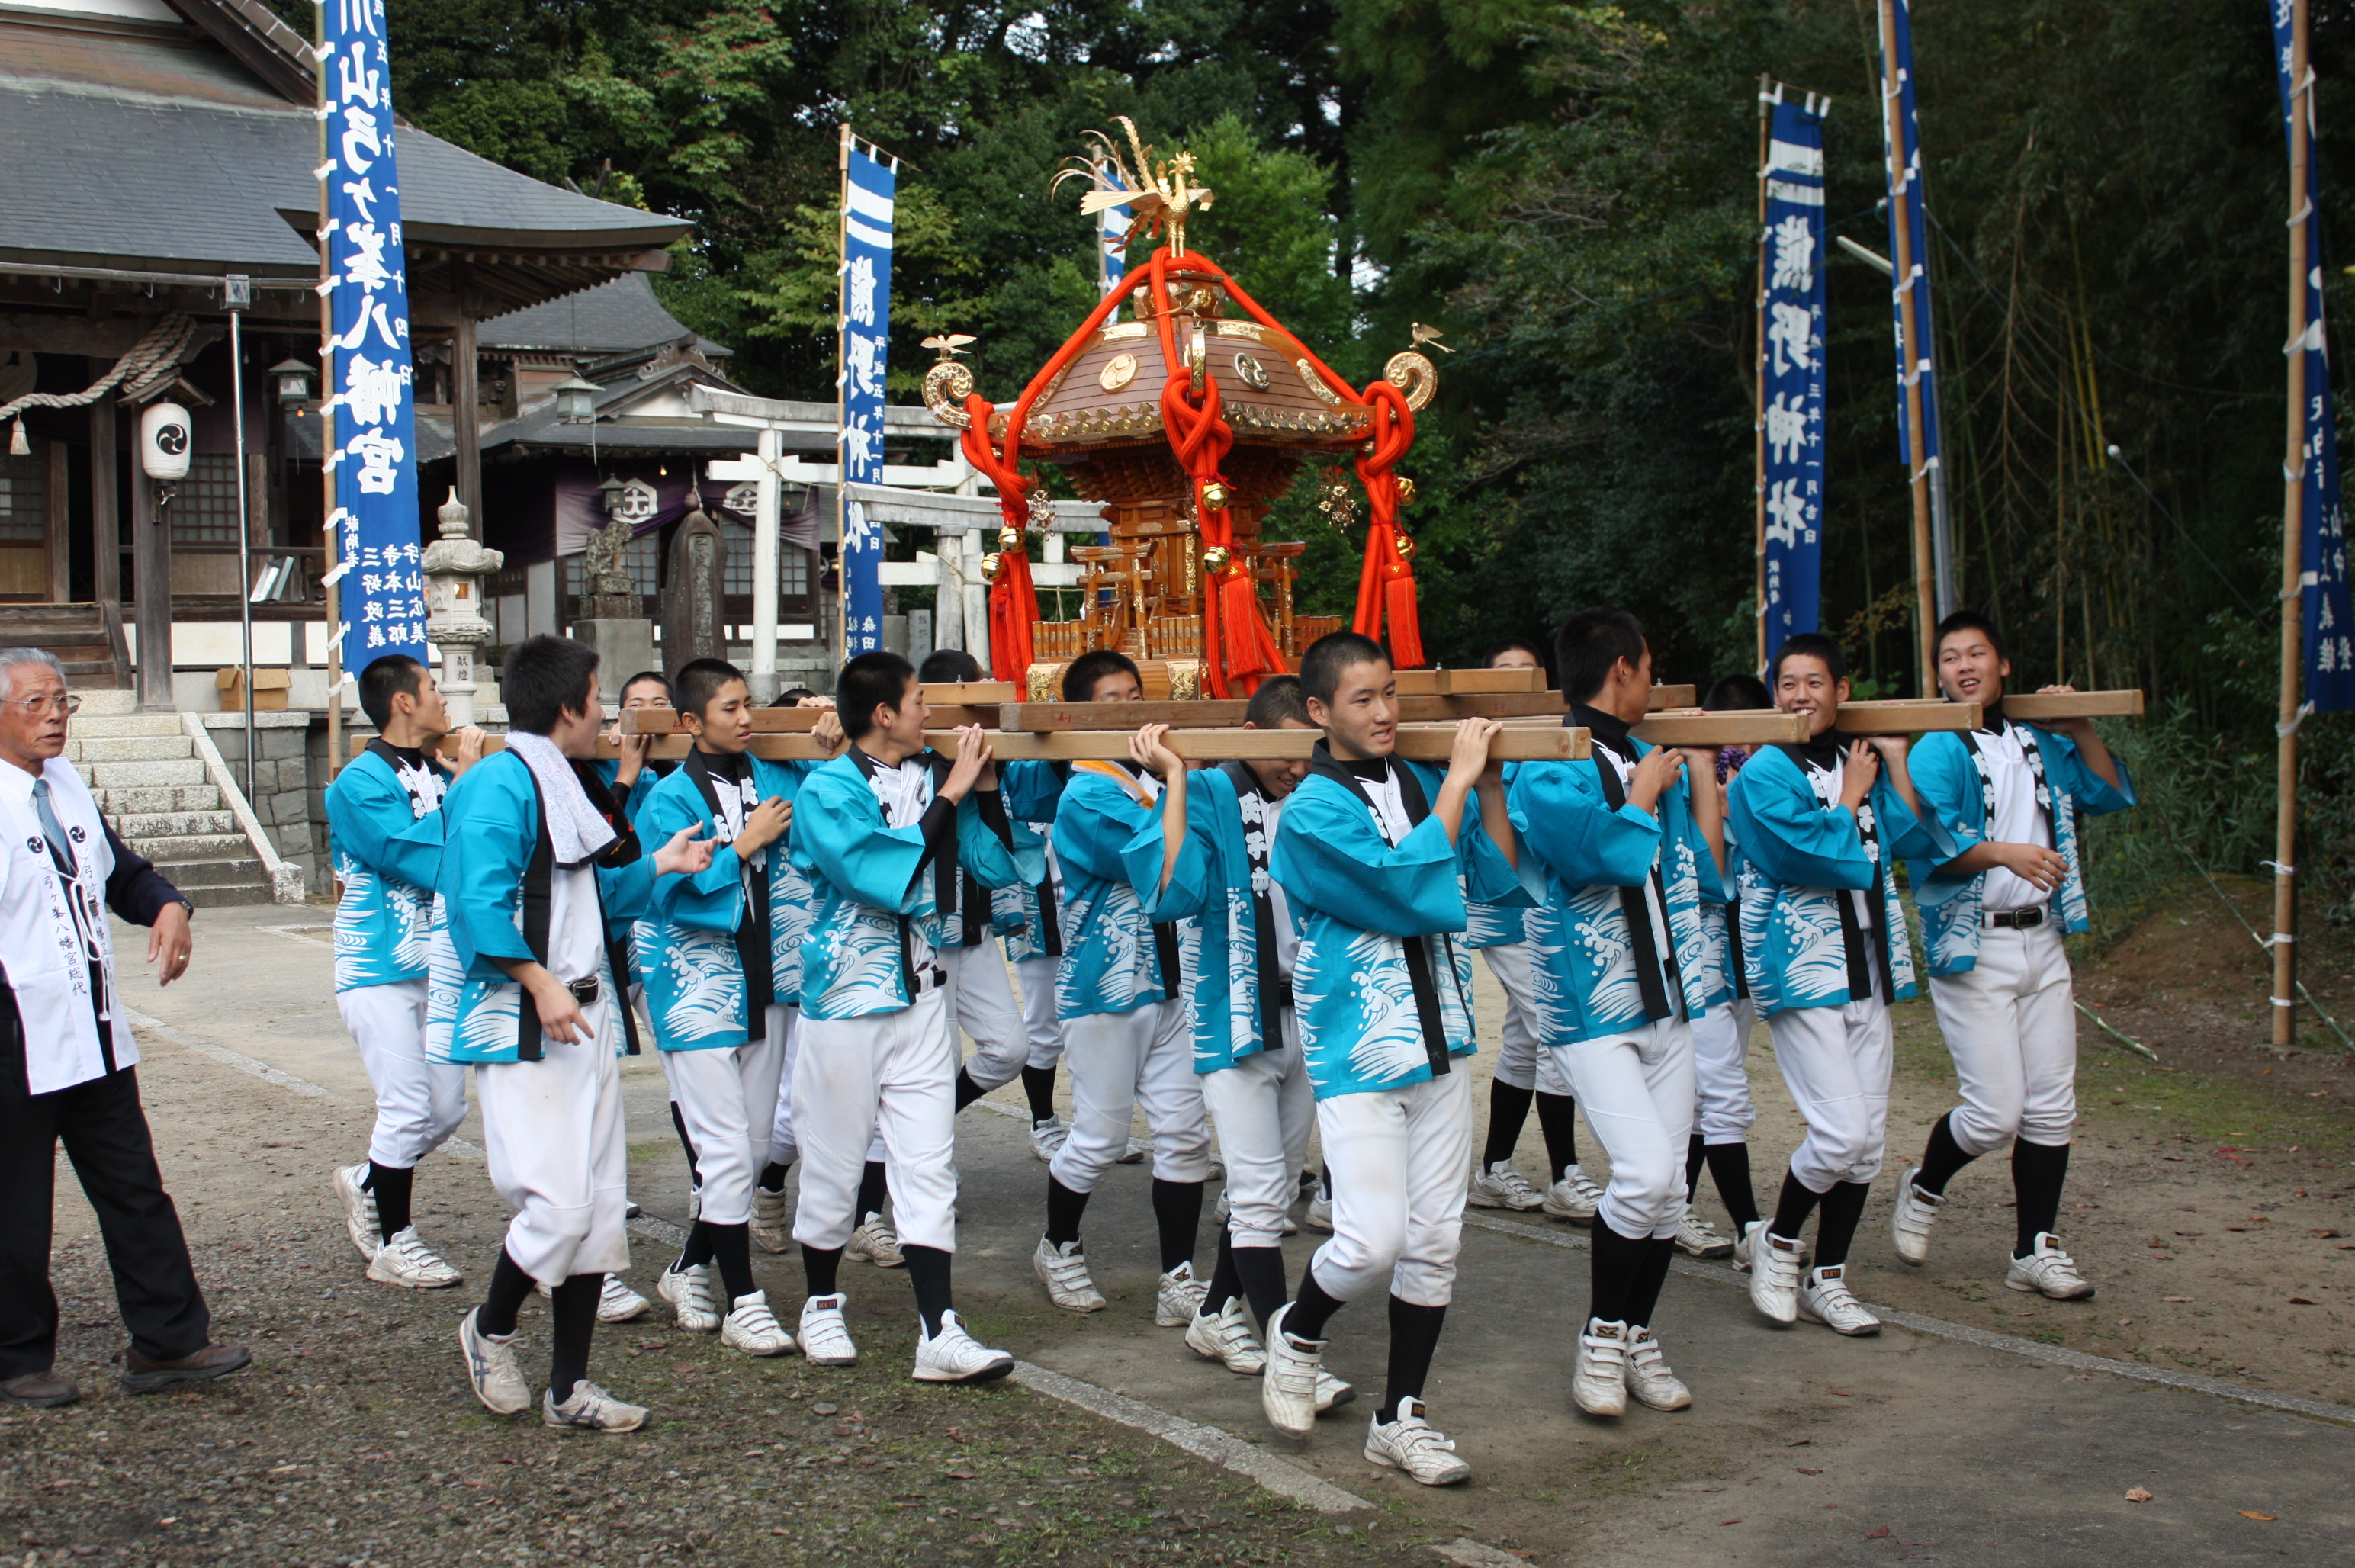
\includegraphics[scale=0.07]{mikoshi.jpg}
	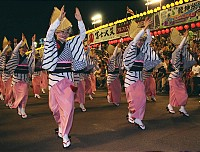
\includegraphics[scale=1.3]{odori.jpg}
\end{center}

\paragraph{} Dans les plus grands Matsuris, de grands chars défilent à travers
le quartier accompagnés des flûtes, tambours et gongs. Ces chars sont aussi
accompagnés de troupes de danseurs. Les filles profitent de ces festivals pour
sortir leurs kimonos pour rentrer dans l'ambiance de la fête.

\begin{center}
	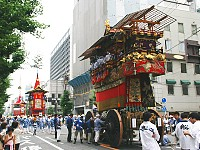
\includegraphics[scale=1.3]{gion.jpg}
\end{center}

\newpage

\section{Matsuris les plus connus}

\begin{itemize}
	\item Aoi Matsuri, 15 mai, Kyoto
	\item Aomori Nebuta Matsuri, 2--7 août, Aomori
	\item Awa-Odori, 12--15 août, Tokushima
	\item Danjiri Matsuri, deuxième week-end de septembre, Kishiwada
	\item Etchu Owara Kaze no Bon, 1--3 septembre Toyama
	\item Gion Matsuri, juillet, Kyoto quartier de Gion
	\item Gozan no Okuribi, 16 août, Kyoto
	\item Hadaka Matsuri, troisième samedi de février, Okayama
	\item Hakata Gion Yamakasa, 1--15 juillet, Hakata
	\item Ise-jingu kannamesai et Ninamesai, 15--25 octobre et 23--29 novembre, Ise
	\item Jidai Matsuri, 22 octobre, Kyoto
	\item Kanda Matsuri, deuxième dimanche de mai, Tokyo
	\item Namahage, 31 décembre, Oga
	\item Narita-san Setsubun-e, 3 février, Narita
	\item Onbashira, avril tous les six ans, Suwa
	\item Otaue Matsuri, 14 juin, Osaka
	\item Sanja Matsuri, troisième week-end de mai, Tokyo
	\item Sanno Matsuri, 14--15 avril, Takayama
	\item Sendai Tanabata Matsuri, 6--8 août, Sendai
	\item Sentei-sai, 3--4 mai, Shimonoseki
	\item Festival de la neige de Sapporo, mi-février, Sapporo
	\item Tenjin Matsuri, 24--25 juillet, Osaka
	\item Yosakoi Matsuri, 9--12 août, Kochi
\end{itemize}

\chapter{Les elfes}
